%%%%%%%%%%%%%%%%%%%%%%%%%%%%%%%%%%%%%%%%%%%%%%%%%%%%%%%%%%%%%%%%%%%%%%%%%%%%
%%%%%                          ANNEXE 1                               %%%%%%
%%%%%%%%%%%%%%%%%%%%%%%%%%%%%%%%%%%%%%%%%%%%%%%%%%%%%%%%%%%%%%%%%%%%%%%%%%%%

\appendix
\renewcommand\chaptername{Annexe~}
\phantomsection 

\lhead[\fancyplain{}{\leftmark}]%Pour les pages paires \bfseries
      {\fancyplain{}{}} %Pour les pages impaires
\chead[\fancyplain{}{}]%
      {\fancyplain{}{}}
\rhead[\fancyplain{}{}]%Pour les pages paires 
      {\fancyplain{}{\rightmark}}%Pour les pages impaires \bfseries
\lfoot[\fancyplain{}{}]%
      {\fancyplain{}{}}
\cfoot[\fancyplain{}{\thepage}]%\bfseries
      {\fancyplain{}{\thepage}} %\bfseries
\rfoot[\fancyplain{}{}]%
     {\fancyplain{}{\scriptsize}}

%%%%%%%%%%%%%%%%%%%%%%%%%%%%%%%%%%%%%%%%%%%%%%%%%%%%%%%%%%%%%%%%%%%%%%%%%%
%%%%%                      Start part here                          %%%%%%
%%%%%%%%%%%%%%%%%%%%%%%%%%%%%%%%%%%%%%%%%%%%%%%%%%%%%%%%%%%%%%%%%%%%%%%%%%
\chapter{PyFast, un outil pour les post-traiter tous}
\label{appendix/pyfast}

%==============================================================================	Résumé du chapitre

\begin{center}
\rule{0.8\linewidth}{.5pt}
\begin{minipage}{0.8\linewidth}
\smallskip

\textit{Cette annexe présente l'outil de post-traitement développé pendant la thèse : PyFast. Son fonctionnement est détaillé avec une attention toute particulière portée sur les schémas d'interpolation et de dérivation, la méthode de détection des tourbillons quasi longitudinaux et la manière d'obtenir les densités spectrales.}

%\smallskip
\end{minipage}
\smallskip
\rule{0.8\linewidth}{.5pt}
\end{center}

\newpage

Un outil a été développé par \cite{Bouillon_PhDThesis} lors de sa thèse, et enrichi avec les thèses de \cite{Doche_PhDThesis} et \cite{Bauer_PhDThesis} pour post traiter les résultats de MULTIFAST. Cet outil de post-traitement permet de calculer des statistiques telles que les vitesses moyennes, les RMS, les facteurs de dissymétrie, etc ; des statistiques d'ordre plus élevé, telles que les termes de transport des contraintes de Reynolds ou de la variance d'un scalaire passif ; allant jusqu'à l'identification des structures tourbillonnaires et l'obtention des densités spectrales. Les statistiques sont ensuite sauvegardées et il faut un outil supplémentaire pour les tracer.\\

Bien que l'outil soit robuste, car validé au cours de plusieurs thèses, il possédait plusieurs défauts liés en grande majorité à la direction utilisée par défaut pour calculer toutes les statistiques. De plus, l'outil aurait nécessité une refonte totale pour qu'il soit utilisé dans la thèse avec le spot transitionnel ou avec la méthode des frontières immergées. Au lieu de modifier le code, le choix a été fait de développer un nouvel outil de post-traitement en Python : PyFast. Il permet de calculer les mêmes statistiques que l'outil Fortran déjà existant sans les limitations évoquées plus haut ainsi que de tracer toutes les statistiques dans un framework personnalisé. De plus, l'outil est compatible avec l'application de visualisation open-source Paraview. Cet outil a été codé en orienté objet et est organisé en plusieurs classes. Le code développé au cours de la thèse est disponible sur le dépôt git: \href{https://github.com/Benji12358/PyFast}{github.com/PyFast}. Un schéma présentant le fonctionnement du code est disponible en \cref{fig/presentation_PyFast}.

\begin{figure}[!hbtp]
    \centering
    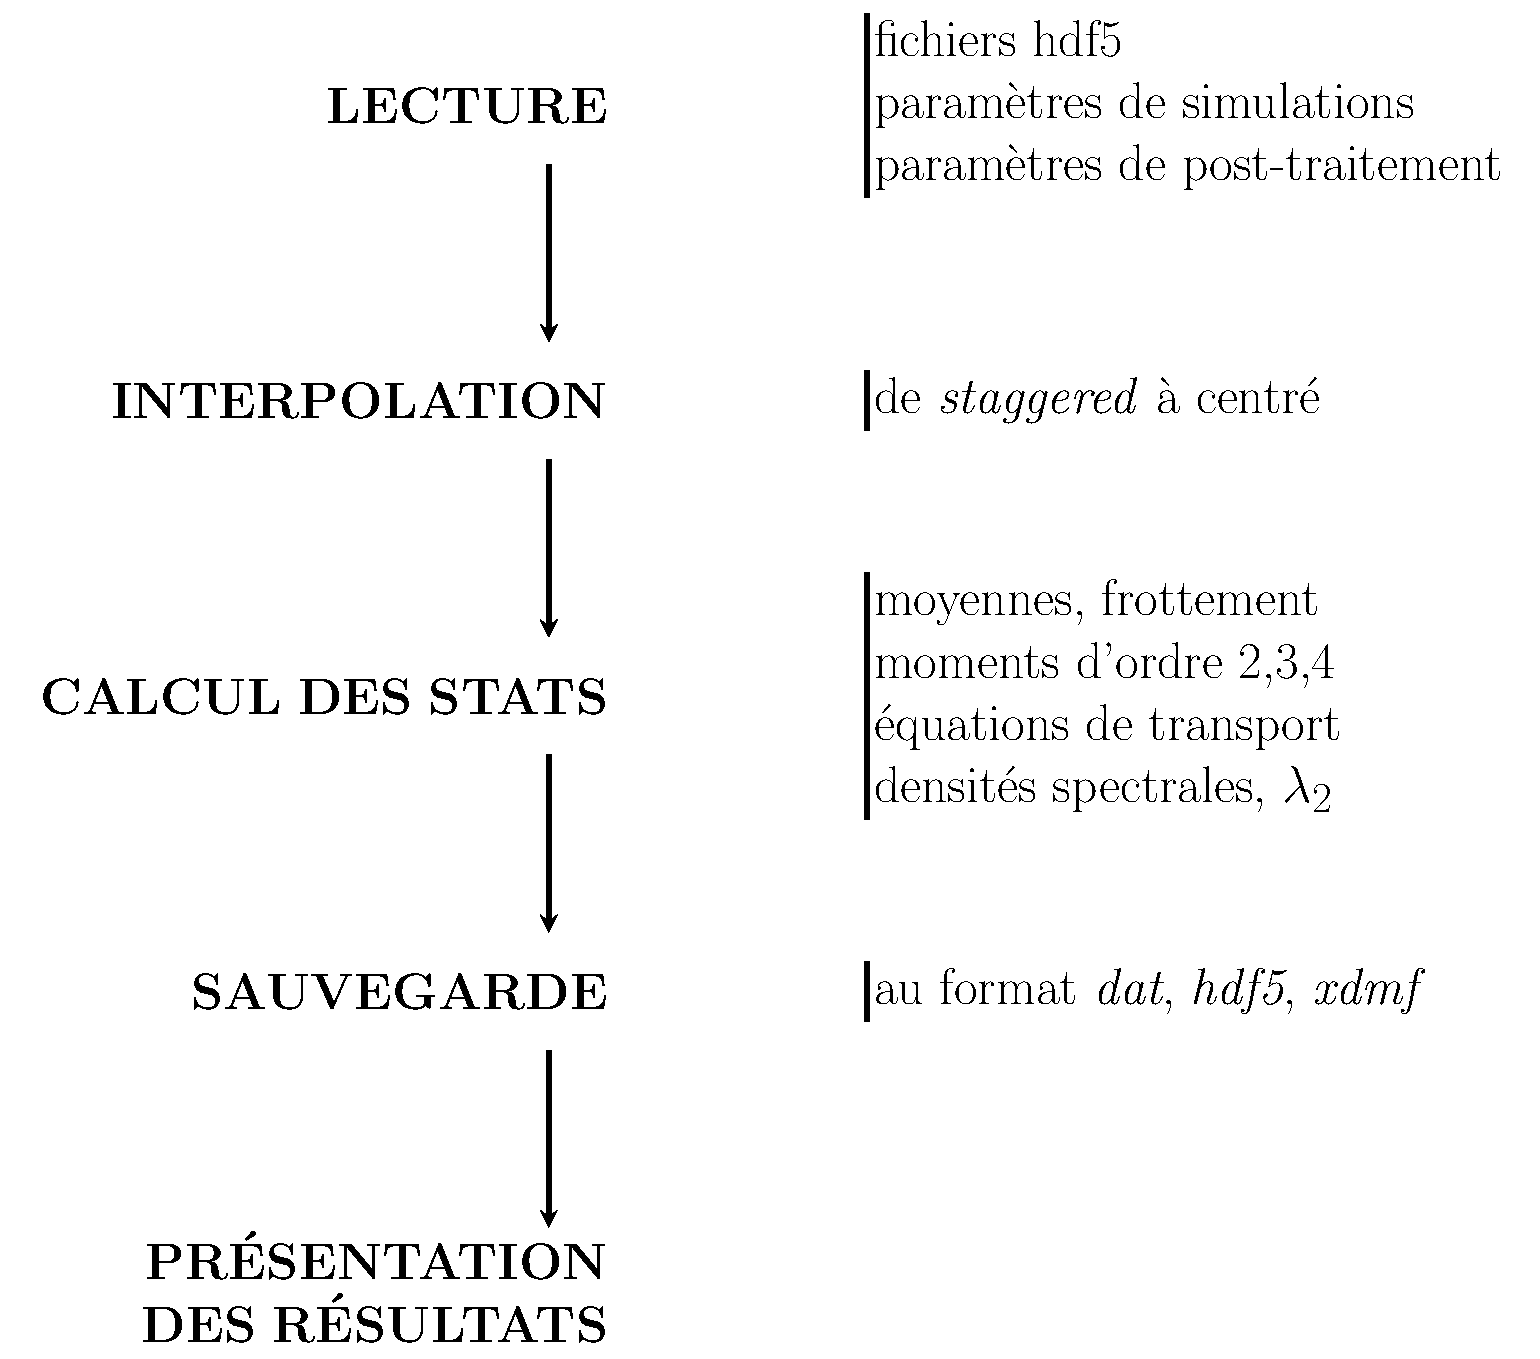
\includegraphics[width=0.75\linewidth]{Annexes/Pictures/Annexe1/presentation_PyFast.pdf}
    \caption{Fonctionnement de l'outil de post-traitement PyFast.}
    \label{fig/presentation_PyFast}
\end{figure}

\clearpage
\section{Schémas d'interpolation et de dérivation}

\begin{figure}[!hbtp]
    \centering
    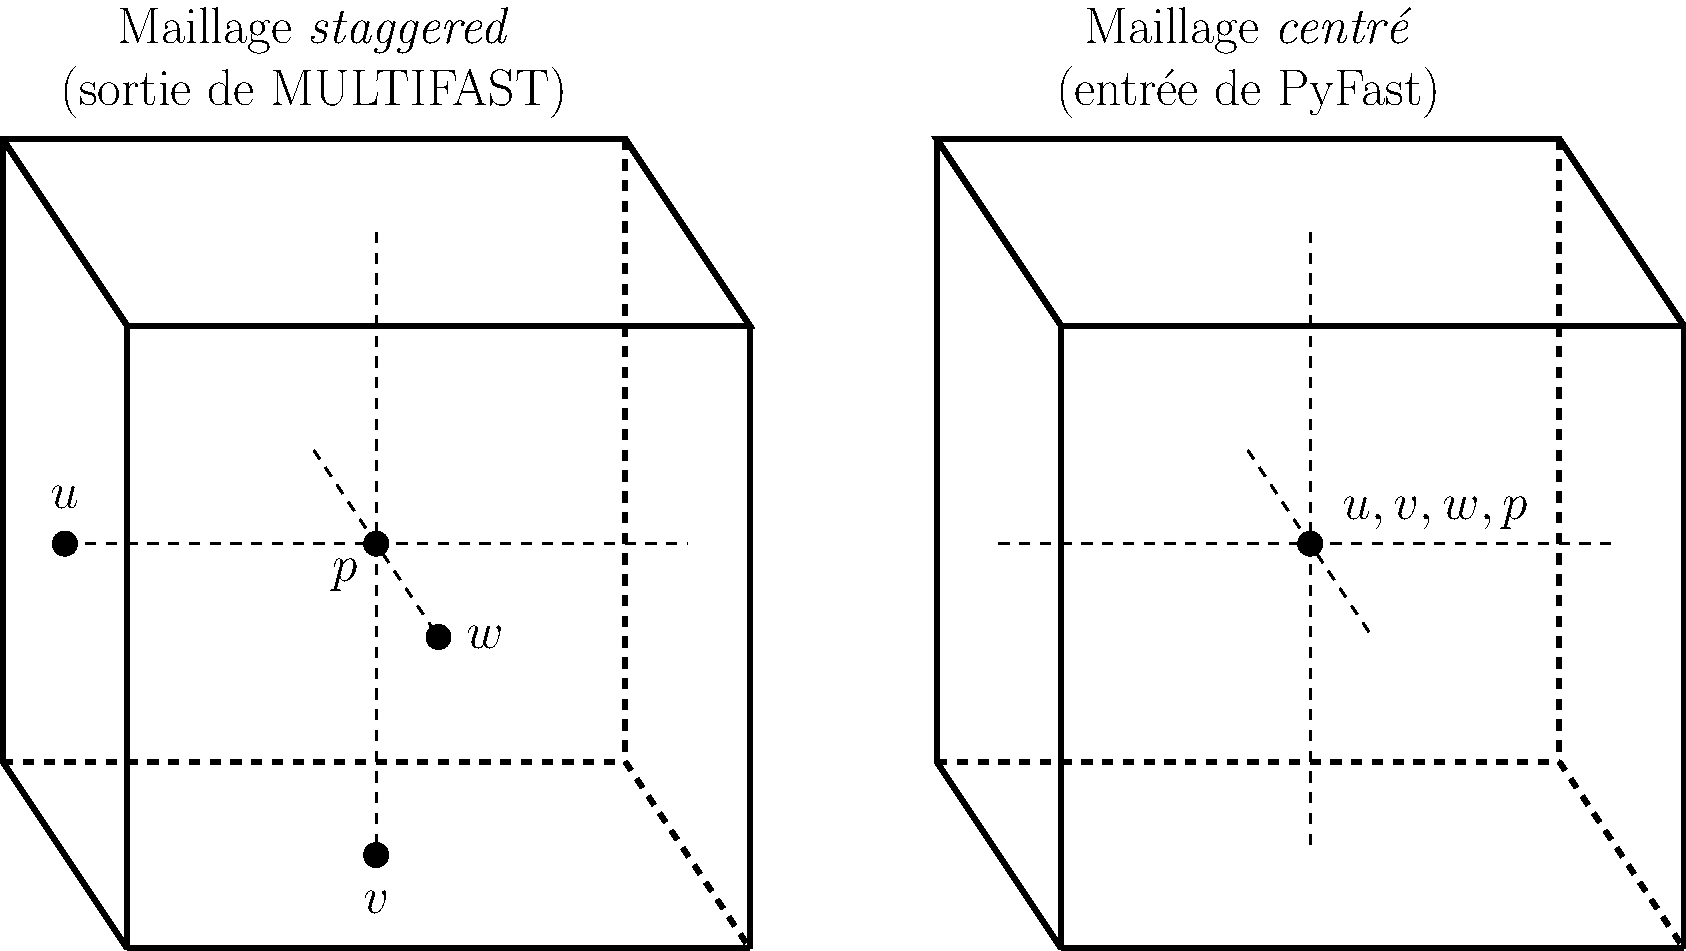
\includegraphics[width=0.7\linewidth]{Annexes/Pictures/Annexe1/node_PyFast.pdf}
    \caption{Passage du maillage \textit{staggered} de MULTIFAST à un maillage \textit{centré} pour PyFast.}
    \label{fig/node_PyFast}
\end{figure}

Les vitesses $u,v$ et $w$ et la pression $p$ sont arrangées sur un nœud de maillage de type \foreignquote{french}{\textit{staggered}} dans MULTIFAST. Dans PyFast, le maillage de type \foreignquote{french}{\textit{staggered}} est d'abord transformé en maillage centré de telle sorte que toutes les vitesses et la pression soient situées au centre du noeud de maillage (\cref{fig/node_PyFast}) pour faciliter le calcul des différentes dérivées nécessaires aux statistiques. La transformation s'effectue grâce à des schémas d'interpolation d'ordre $2$. En reprenant la notation introduite dans le chapitre 2, l'interpolation de la variable $f$ dans une direction uniforme $x$ avec le pas spatial $\Delta x$ s'écrit  :

\begin{equation}
    f \left( x_{0} + \frac{\Delta x}{2} \right) = \frac{f(x_{0})+f(x_{0}+\Delta x)}{2} + \mathcal{O}(\Delta x^{2})
\end{equation}

\subsection{Schémas de dérivation}

Des schémas d'ordre $2$ de type centré sont utilisés pour la dérivation. Toujours avec la notation introduite en chapitre 2, la dérivée première de la variable $f$ dans une direction uniforme $x$ avec le pas spatial $\Delta x$ s'écrit :

\begin{equation}
    \left. \frac{\partial f}{\partial x} \right|_{x_{0}} = \frac{f(x_{0}+\Delta x)-f(x_{0}-\Delta x)}{2 \Delta x} + \mathcal{O}(\Delta x^{2})
\end{equation}

et sa dérivée seconde :

\begin{equation}
    \left. \frac{\partial^{2} f}{\partial x^{2}} \right|_{x_{0}} = \frac{f(x_{0}+\Delta x)-2 f(x_{0})+f(x_{0}-\Delta x)}{\Delta x^{2}} + \mathcal{O}(\Delta x^{2})
\end{equation}

Les dérivées sont calculées grâce à la fonction \textit{gradient} de la librairie Python \textit{numpy} dans PyFast, ce qui présente l'avantage de pouvoir calculer les dérivées dans des directions non homogènes.

%%%%%%%%%%%%%%%%%%%%%%%%%%%%%%%%%%%%%%%%%%%%%%%%%%%%%%%%%%%%%%%%%%%%%%%%%%%%%%%%%%%%%%%%%%%%
\clearpage
\section{Calcul des statistiques}

Toutes les statistiques sont calculées dans un volume de contrôle, en considérant les directions $x$ et $z$ homogènes. Utiliser un volume de contrôle permet d'exclure certaines parties du canal, et de ne calculer les statistiques que localement. Cela est surtout utilisé pour les simulations avec le spot transitionnel, ainsi que celles avec les frontières immergées. Bien entendu, pour un canal turbulent classique, le volume de contrôle est le canal entier. \\

Les statistiques peuvent être moyennées uniquement en espace (dans le cadre de l'étude du spot transitionnel) ou en temps et en espace (pour les canaux turbulents classiques ou les simulations avec les frontières immergées). Toutes les fonctions créées pour calculer les statistiques se trouvent dans la classe \textit{CFD stats}. 


\subsection{Détection de structures cohérentes et TQLs}

Parmi toutes les statistiques calculées avec PyFast, la détection de structures cohérentes et de TQLs demande plus d'attention et d'explication. Les structures cohérentes dans l'écoulement sont détectées avec la méthode $\lambda_{2}$ de \citet{Jeong1995}. Des tourbillons quasi longitudinaux (TQLs) se trouvent parmi ces structures cohérentes. Il y a également la nécessité de les détecter. Pour ce faire, les $\lambda_{2}$ de l'écoulement sont tout d'abord calculés avec les fluctuations de vitesse. Ensuite, les minimums locaux de $\lambda_{2}$ sont détectés dans des plans $y-z$, pour chaque $x$ grâce à la librairie Python \textit{scipy} et la fonction \textit{filters}. Chaque structure cohérente, et donc chaque TQL, est alors représenté par une ligne unique de minimums locaux. Un point important à préciser est que la détection des minimums locaux ne garde que les structures étant dans le sens longitudinal. Pour détecter les TQLs, il suffit de parcourir chaque ligne unique de minimums locaux et de calculer sa longueur et son inclinaison. Pour rappel, un TQL est une structure tourbillonnaire très peu inclinée et allongée dans le sens de l'écoulement. Bien entendu, dans le code la ligne unique de minimum locaux est discrétisée entre $i_{s}$ et $i_{e}$, ce qui change légèrement l'algorithme de détection des TQLs.\\

Pour chaque point $(i_{0})$ de la ligne, en commençant par $i_{s}$, le prochain point $(i_{0}+1)$ de la ligne est identifié. Si ce point respecte le critère d'inclinaison, alors il est retenu et l'opération est répétée avec le prochain voisin. Lorsque la condition d'inclinaison n'est plus respectée, il faut calculer la taille de structure entre les points $i_{s}$ (début de la structure cohérente) et $(i_{0})$ (dernier point respectant le critère d'inclinaison). Si la taille est supérieure à $l^{+}_{x}=150$ alors le centre de la structure cohérente est sauvegardé dans la liste des TQLs. Si tous les points de la ligne unique de minimums locaux respectent le critère d'inclinaison, alors la taille de la structure est calculée entre $i_{s}$ et $i_{e}$.\\

\begin{figure}[!hbtp]
    \centering
    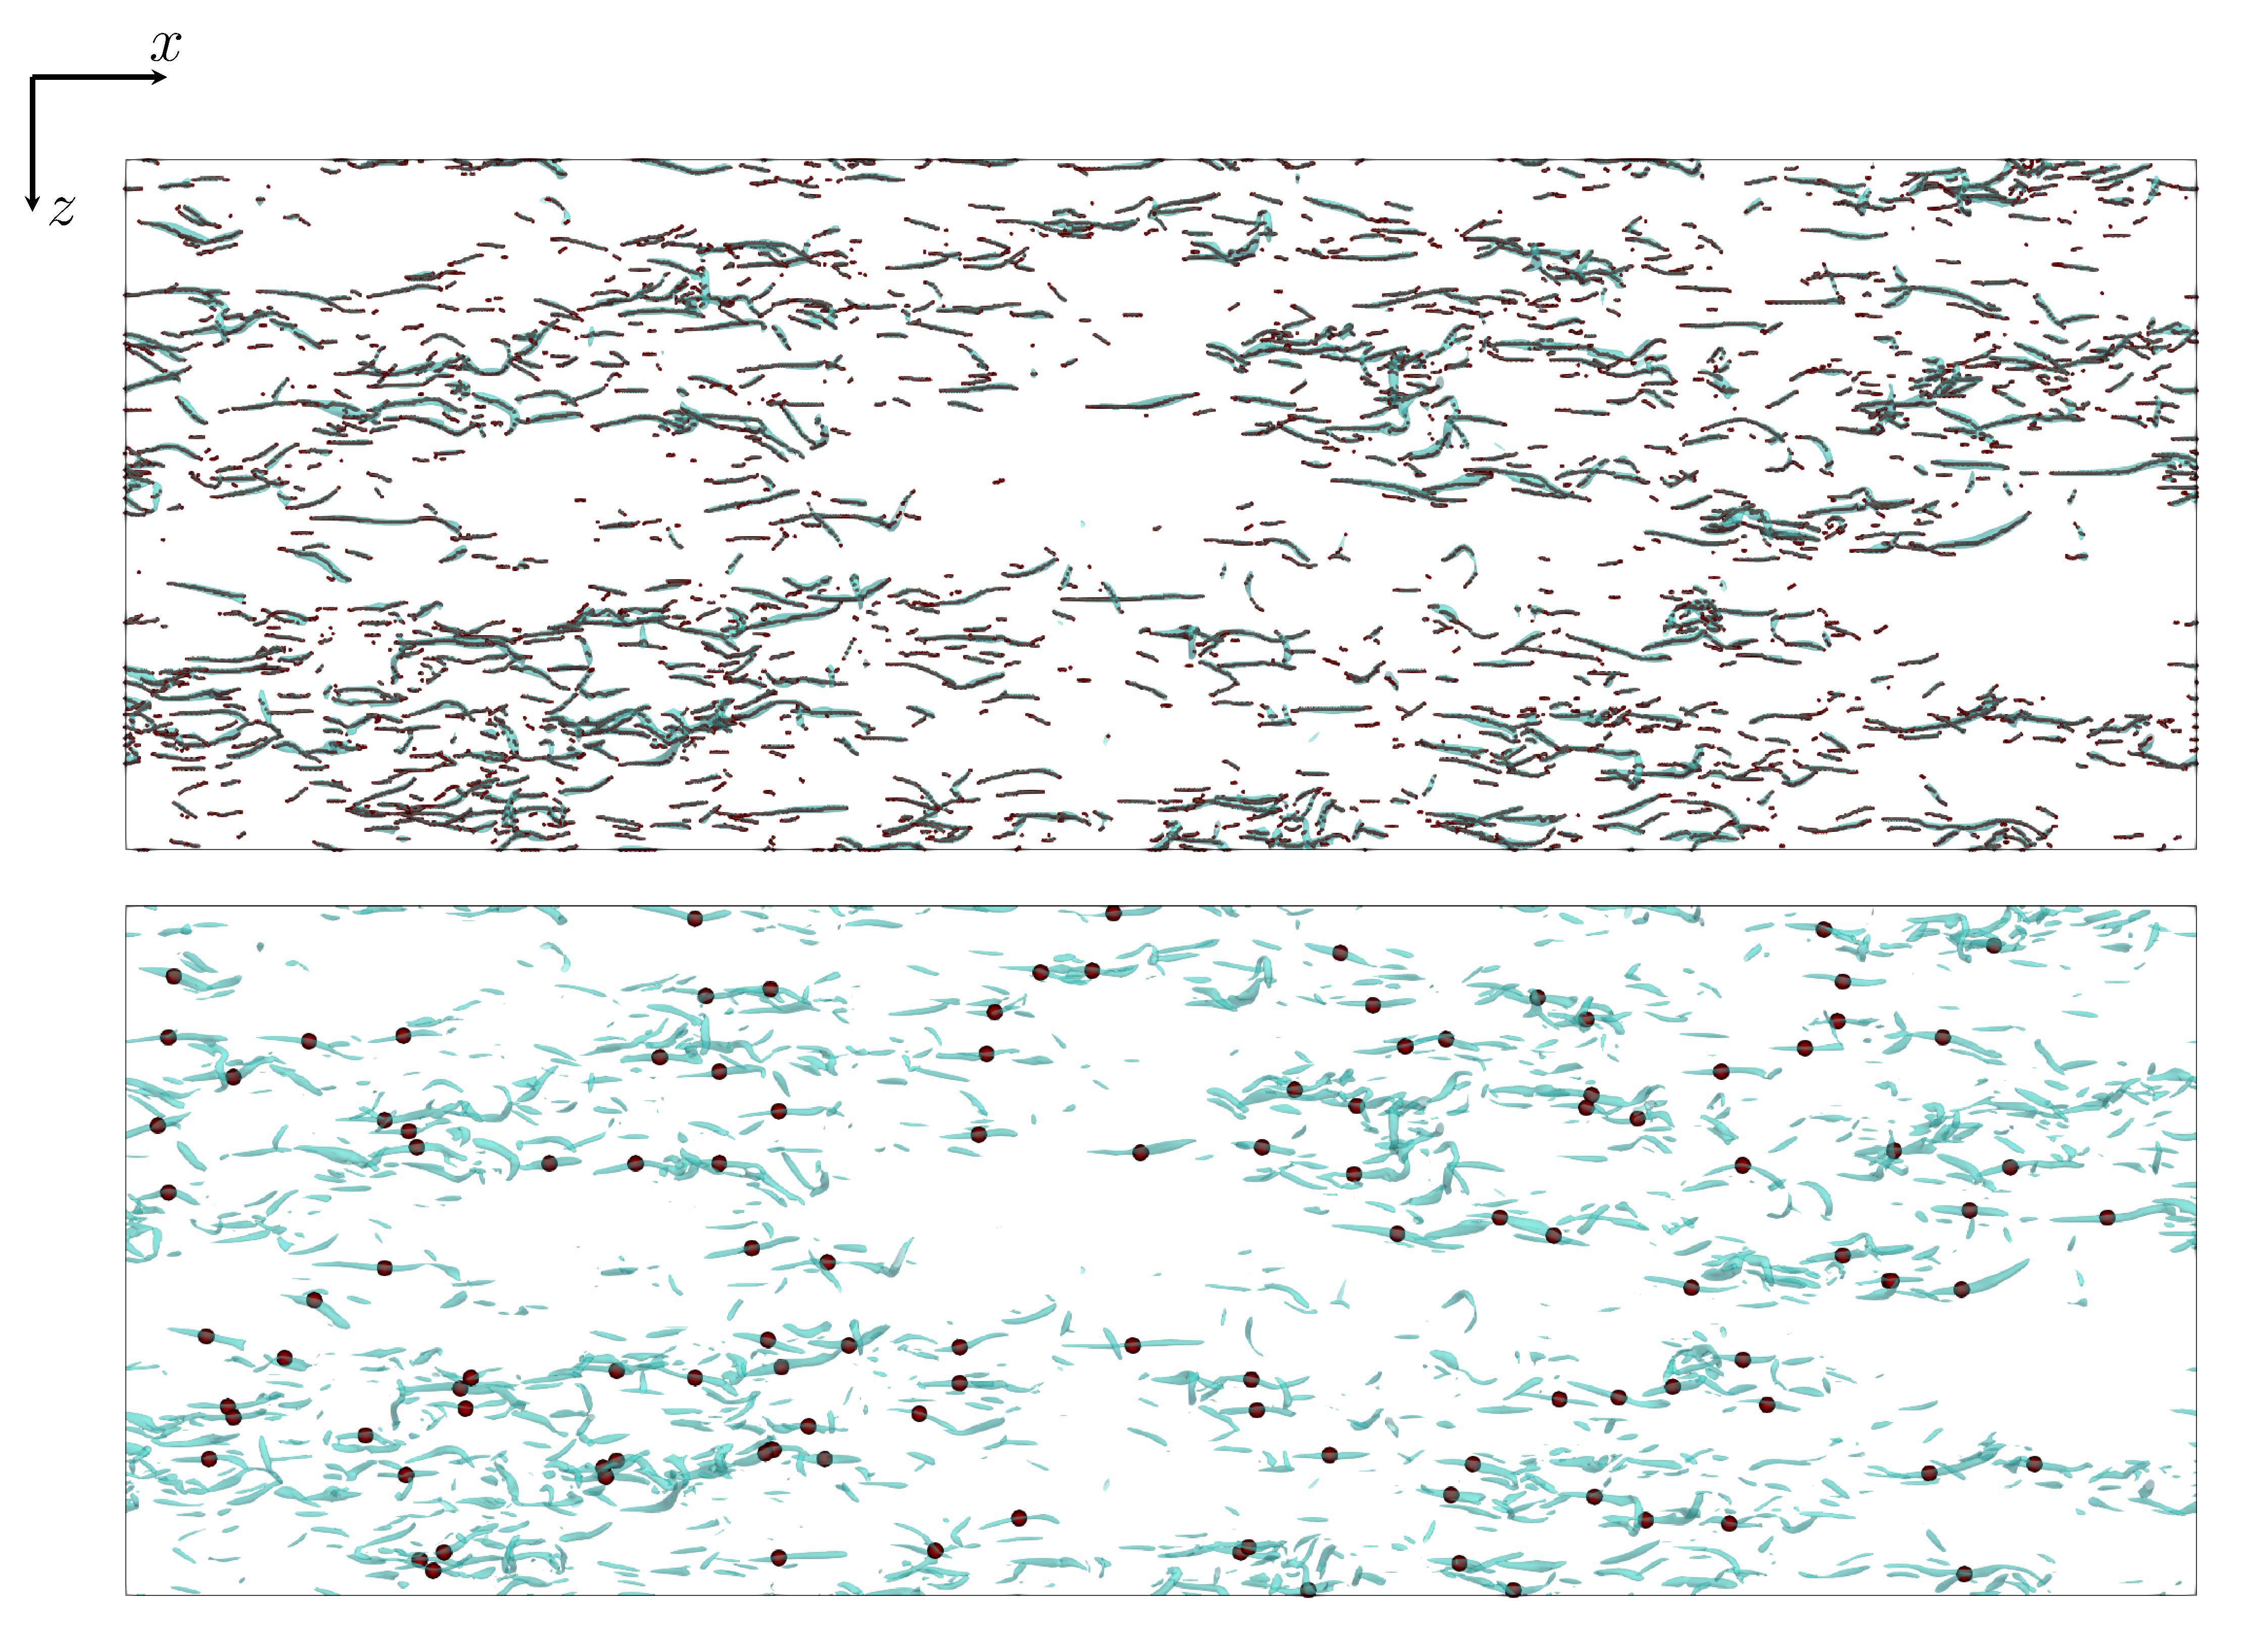
\includegraphics[width=\linewidth]{Annexes/Pictures/Annexe1/Detection_TQL.pdf}
    \caption{Exemple d'application de l'algorithme de détection des TQLs. Les contours des $\lambda_{2}=-0.02$ sont tracés en cyan dans la partie inférieure du canal. \refInFig{en haut} minimums locaux de $\lambda_{2}$, \refInFig{en bas} centres des TQLs détectés, tous deux représentés par des points rouges.}
    \label{fig/Detection_TQL}
\end{figure}

\clearpage
La \cref{fig/Detection_TQL} montre un exemple d'application de l'algorithme sur un champ instantané de la simulation utilisée pour valider MULTIFAST. Les contours de $\lambda_{2}=-0.02$ sont tracés en cyan et les minimums locaux, ainsi que les centres des TQLs détectés, sont représentés par des points rouges. La densité de probabilité des TQLs a été tracé pour le cas d'un canal turbulent pour valider l'approche utilisée pour détecter les TQLs. La courbe obtenue est semblable à celle de \citet{Gallorini2022}, et le maximum de la courbe est atteint à une position similaire que celle trouvée par \citet{Jeong1997}. La technique de détection est donc validée, mais reste néanmoins sensible aux paramètres initiaux (taille minimale et inclinaison maximum des TQLs). 

\subsection{Transformation de Fourier et fonction de fenêtrage}

Les transformées de Fourier 2D sont calculées grâce à la librairie Python \textit{numpy} et sa fonction \textit{fft2}. Elle est ensuite multipliée par son conjugué, et prémultipliée par $k_{x}$ et $k_{z}$ pour obtenir les densités spectrales présentées dans le manuscrit. Dans le cas d'un canal turbulent développé, les densités spectrales sont similaires à celles obtenues par \citet{Bauer_PhDThesis}.\\

Les fonctions de fenêtrage permettent d'isoler une partie du champ global. Du bruit artificiel serait ajouté aux transformées de Fourier calculées sans fonction de fenêtrage. Elles sont donc nécessaires dans le cadre de l'étude du spot transitionnel où les densités spectrales ont été calculées dans le cœur turbulent grâce à une fonction de type Hann :

\begin{equation}
    h(t) = \left\{ \begin{array}{lll}
    0.5 - 0.5 \times cos\left( \frac{2 \pi t}{T} \right) && \text{ si } t \in [0,T],\\
    0 && \text{ sinon}.
    \end{array} \right.
\end{equation}

La fonction de fenêtrage est multipliée au champ brut au moment de calculer la transformée de Fourier dans PyFast.

\section{Sauvegarde et présentation des statistiques}

Le calcul et la présentation des statistiques sous forme de graphes est effectué dans deux parties différentes, comme pour le code de post-traitement initial. Une fois les statistiques calculées, elles sont sauvegardées au format \textit{csv} dans un fichier \textit{dat} comportant une description du fichier en entête. La sauvegarde des densités spectrales est effectuée dans un fichier \textit{hdf5}. Enfin, les champs $\lambda_{2}$ ou les éventuels champs à visualiser avec Paraview, sont sauvegardés conjointement dans un fichier \textit{hdf5} (pour les données brutes) et dans un fichier \textit{xdmf} (pour décrire la structure des données).\\

Finalement, la librairie Python \textit{matplotlib} a été instanciée pour tracer les statistiques. Toutes les fonctions aidant à l'obtention de graphes se trouvent dans la classe \textit{CFD plot}.
